\chapter{Architecture}
\label{ch:architecture}

\begin{quotation}
“The greatest pleasure in life is doing what people say you cannot do.”
{\small\it -- Walter Bagehot (British political Analyst, Economist and Editor, one of the most influential journalists of the mid-Victorian period.1826-1877) }
\end{quotation}

In this section we explain the overall architecture of the system and the architecture proposal of the solution for the problem presented in distributed data stores regarding consistency versus availability. Rather than considering just a fixed consistency model, we aim to providing finer-grained levels of consistency during the replication of items. For that, will be explored how bounded data semantics help to achieve that goal. First of all, we take a general overview of the system design in section~\ref{architecture:overview}. Following sections reflect the current architecture of the system in terms of network as well software components. Each of the steps in the design process is justified, and in particular those related to asynchronous replication using RPC mechanism for the architectural changes introduced into HBase with a custom HBase-QoD module. To do that, it is necessary taking into account the main requirements that fulfill our goals as specified in section~\ref{architecture:requirements}. Therefore, we are able to show the logic behind the main architectural design decisions and showcase the main goal scenarios as seen for instance in a "thousand feet" high-level view of the system with Figure~\ref{fig-high-level}. Following and up to the evaluation, we delve into the proposed changes in order to verify the feasibility of the implementation as well as what scenarios are best suited to our definition of consistency.

  %%%%%%%%%%%%%%%%%%%%%%%%%%%%%%%%%%%%%%%%%%%%%%%%%%%%%%%%%%%%%%%%%%%%%%%%%%%%%
  %
%%%%%                        SECTION
 %%%
  %
\section{System overview}\label{architecture:overview}
% How the containers replicate thigns with the QoD
%reprise overall system overview of HBase (if needed check approach in papers such as BigTable or HBAse papers/docs) kind of usage overview, applications, storage, data centers, etc. (the 1000 feet view or birds-eye view)
Given the fact that HBase already provides an eventual consistency mechanisms through Remote Procedure Calls in order to replicate items, we chose that data store as the default system to first implement our proposed architecture. Also, we can enhance the current multi-row atomic model, using an approach that can also relate column families between updates in order to provide the same atomicity at the column-level. That is potentially useful for distinguishing updates between cluster update owners and users or applications that need those updates from another cluster for the fact of being consistently up to date in regards to their own local data center ongoing update operations. The overall architecture layout is presented in Figure~\ref{fig-high-level}. The module that introduces the vector-field consistency model is shown in Algorithm~\ref{algo1}, and follows the architectural design choices of HBase as well as the main goals here desired. 

\paragraph{Data Center Storage View:}

%insert 1000 feet view
\begin{figure}[t]
\centering
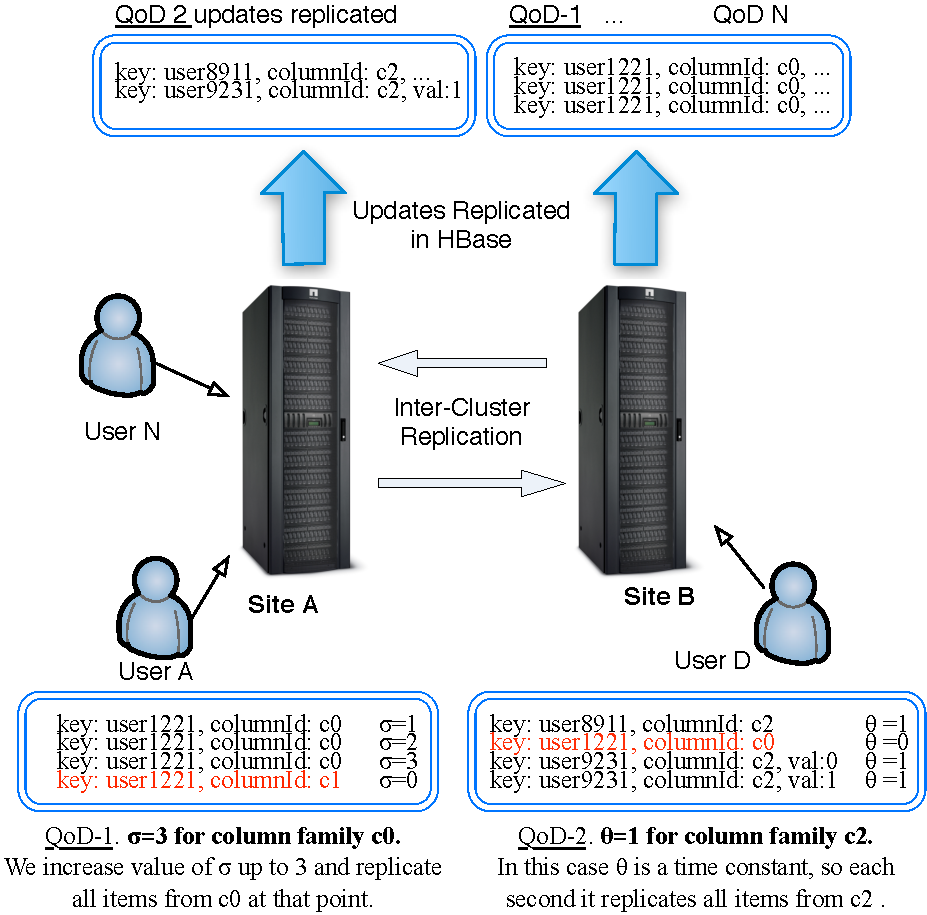
\includegraphics[width=0.8\linewidth]{figs/highlevel.pdf}
\caption{HBase QoD high-level}
\label{fig-high-level}
\end{figure}

\paragraph{Application Flow:}



\paragraph{Usage:}



\section{Network Architecture}
% - diagrams and clear explanations of how HBase and its distribution and replication works within data center and across data centers this is where your diagrams should show up describing the information flows and where QoD is to be applied.  
At the Replication Level, the network architecture is as shown in Figure ~\ref{fig-replication-level}. Which reflects the main components at each site by exposing them into adjacent layers which interact with each other. The flow is both, upwards and downwards the stack in each of the Master servers of HBase in the distributed cluster set up at INESC-ID.

\begin{figure}[t]
\centering
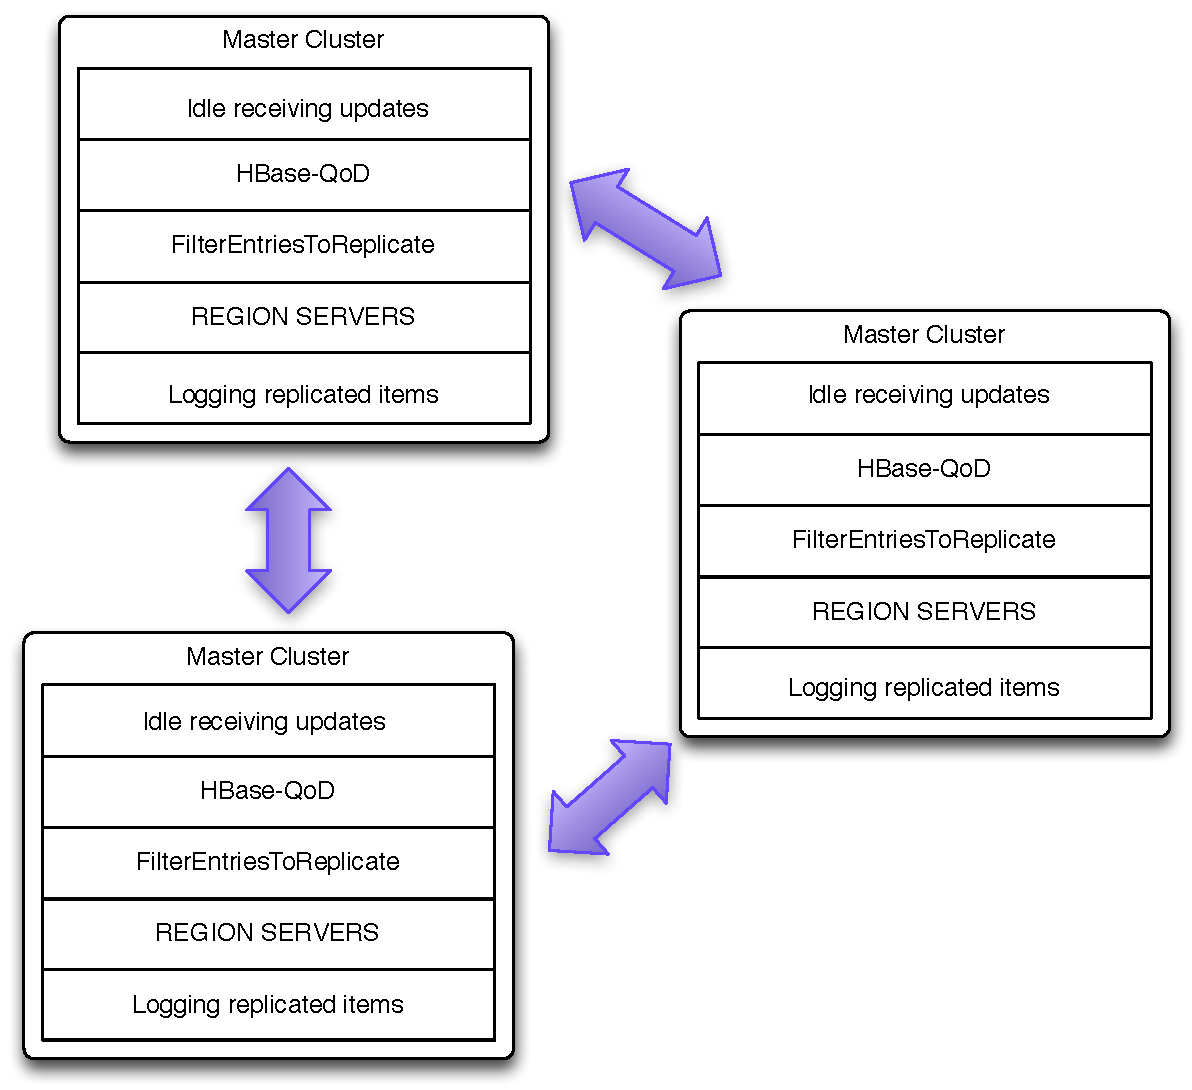
\includegraphics[width=0.8\linewidth]{figs/ReplicationFlow.pdf}
\caption{Replication Flow of updates}
\label{fig-replication-level}
\end{figure}

\section{System Architecture}
% architecture inside each HBase instance with your new modules.
A three-dimensional vector constraint model based on~\cite{Santos:2010} is implemented in the form of the corresponding QoD paradigm, shipping updates for replication, or retaining them for later shipment as mentioned. For that to be possible, we have used a set of customized data structures, which hold the values of the database rows we desire to check according to some specific field we might be interested in (e.g column family) for replication. 

\section{Consistency Enforcement}\label{architecture:consistency}
% description of the VFC algorithms and how the consistency is enforced whan updates arrive , etc. this also includes operation grouping (only code like details should be left for the implamentations, e.g., the listings that you show there and are ok).
%% Start by presenting our model, constraints, data containers, and how things work (are enforced / evaluated )
The QoD paradigm implemented allows for entries to be evaluated prior to replication based on one or several of the three parameters in a three-dimensional vector K ($\theta$, $\sigma$, $\nu$), corresponding to Time, Sequence, Value respectively in our case. Secondly, we take care of updates that collide with previous ones (same keys but different values). They can also be checked for number of pending updates or value difference from previously replicated updates, and then shipped or kept on the data structure accordingly. The time constraint can be always validated every X seconds, and the other two constraints are validated through Algorithm.~\ref{algo1}, whenever updates arrive. For the work presented here we use Sequence ($\sigma$) as the main vector-field bound (\texttt{HBaseQoD.enforce(containerId)}).

% architecture inside each HBase instance with your new modules.
The original HBase architecture has built-in properties derived from the underlying HDFS layer. As part of it, the WALEdit data structure is used to store data temporarily before being replicated, useful to copy data between several HBase locations. The QoD algorithm (shown in Algorithm.~\ref{algo1}) uses that data structure, although we extend it to contain more meaningful information that help us in the management of the outgoing updates marked for replication.

% High-level algorithm we use to modify queued items for replication
\begin{algorithm*}
\caption{QoD high-level algorithm for filtering updates}
\label{algo1}
\begin{algorithmic}[1]
\REQUIRE $containerId$
\ENSURE $maxBound \neq 0$ and $controlBound \neq 0$
%\STATE $y \leftarrow 1$
\WHILE{$enforceQoD (containerId)$}
\IF{$getMaxK(containerId) = 0$}
\RETURN $true$
\ELSE[$getactualK(containerId)$]
\STATE $actualK(\sigma) \leftarrow actualK(\sigma)+1$
	\IF{$actualK(\sigma) \geq containerMaxK(\sigma)$}
	\STATE $actualK(\sigma) \leftarrow 0$
	\RETURN $true$
	\ELSE
	\RETURN $false$
	\ENDIF
\ENDIF
\ENDWHILE
\end{algorithmic}
\end{algorithm*}

To compare and track the QoD fields, that act as constraints to replicate updates, against these stored entries, we defined data \emph{containers} which are useful to keep track of the current value of the vector-field selected to bound replication to, and secondly the maximum value it will be allowed to reach before updates are flushed to the slave cluster and then reset again. That is as what we call the QoD percentage of updates replicated (according to the selected vector-field bound, e.g $\sigma$). The process is partly automated, of by now, we just define it at run-time (or by the developer later) by adding a parameter into the system console to define a vector-field specific bound.

\section{Prototypical Example}
% complete example of usage, that I think you are presenting in the implementation. describe how a client application program  can specifiy the Qod and operationg groupings so that the reader sees everything now in a complete example (this may be shown earlier but I think it is a good way of wrapping up everything and make it more clear)
We extend HBase, adding updates due to be replicated in a priority queue according to their own QoD in each case. Thereafter once the specified QoD threshold is reached another thread from HBase in the form of Remote Procedure Call collects and ships all of them at once.

\begin{figure}[t]
\centering
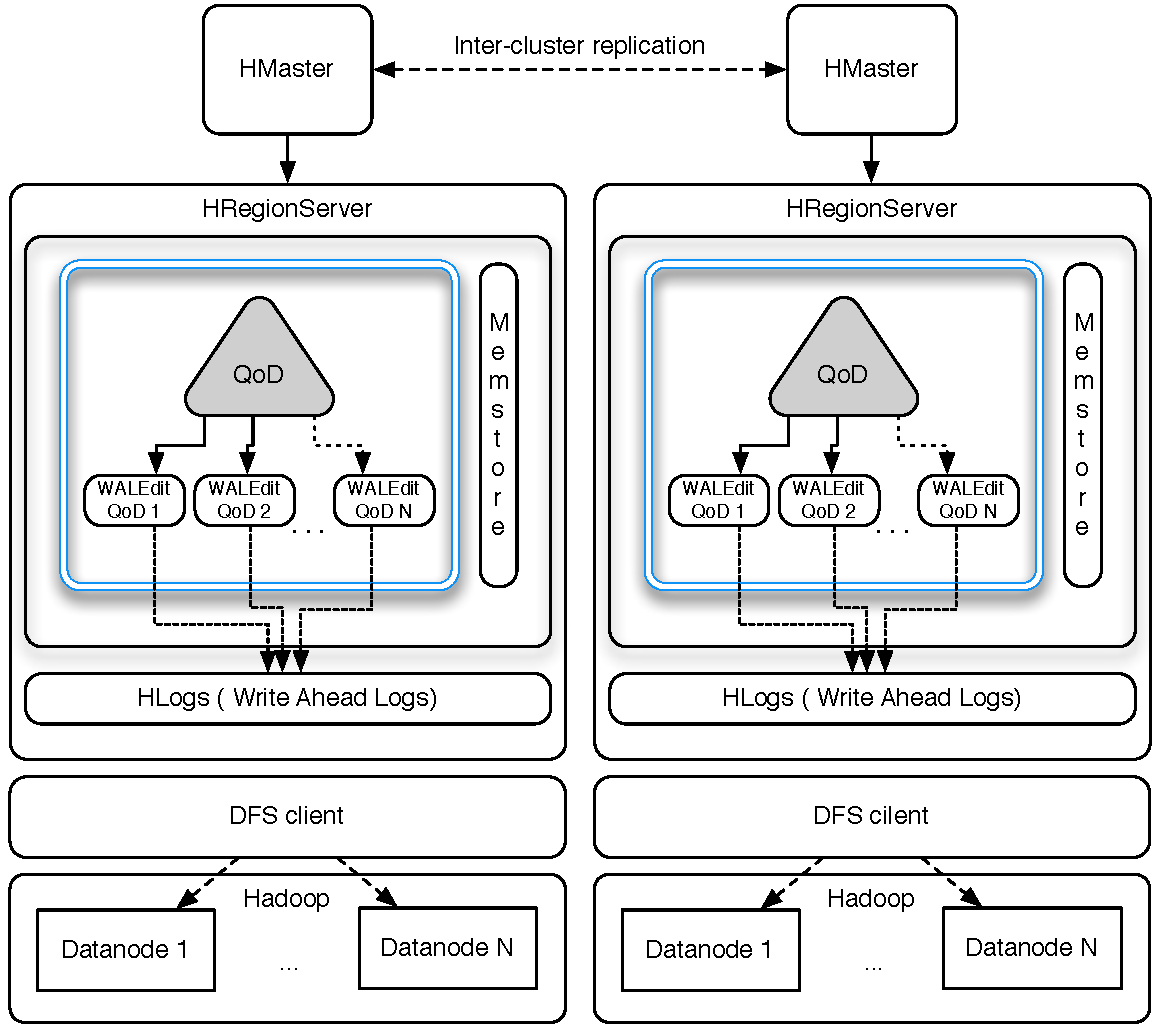
\includegraphics[width=0.8\linewidth]{figs/multi-site.pdf}
\caption{HBase QoD operation}
\label{fig-qod-module}
\end{figure}

In Figure~\ref{fig-qod-module} we observe the QoD module plugging into HBase, intercepting the incoming updates from the upper layers and passing them down and the resulting outcome to the Write Ahead Logs for later replication.

\section{Software Architecture}
%Class Diagram of relevant classes of each HBase instance and your new classes, and classes that have been modified in their interface/methods/public properties.
In the following Figure~\ref{fig-class-diagram} it is depicted the main class diagrams for the architecture solution. Highlighted diagrams in \emph{green} are classes we have introduced into the system or modified in the case of partially highlighted. The main components are the HBaseQoD and the function \emph{filterEntriesToReplicate} where resides the main Algorithm~\ref{algo1} for the consistency enforcement of data semantics we see in \ref{architecture:consistency}.

\begin{figure}
\centering
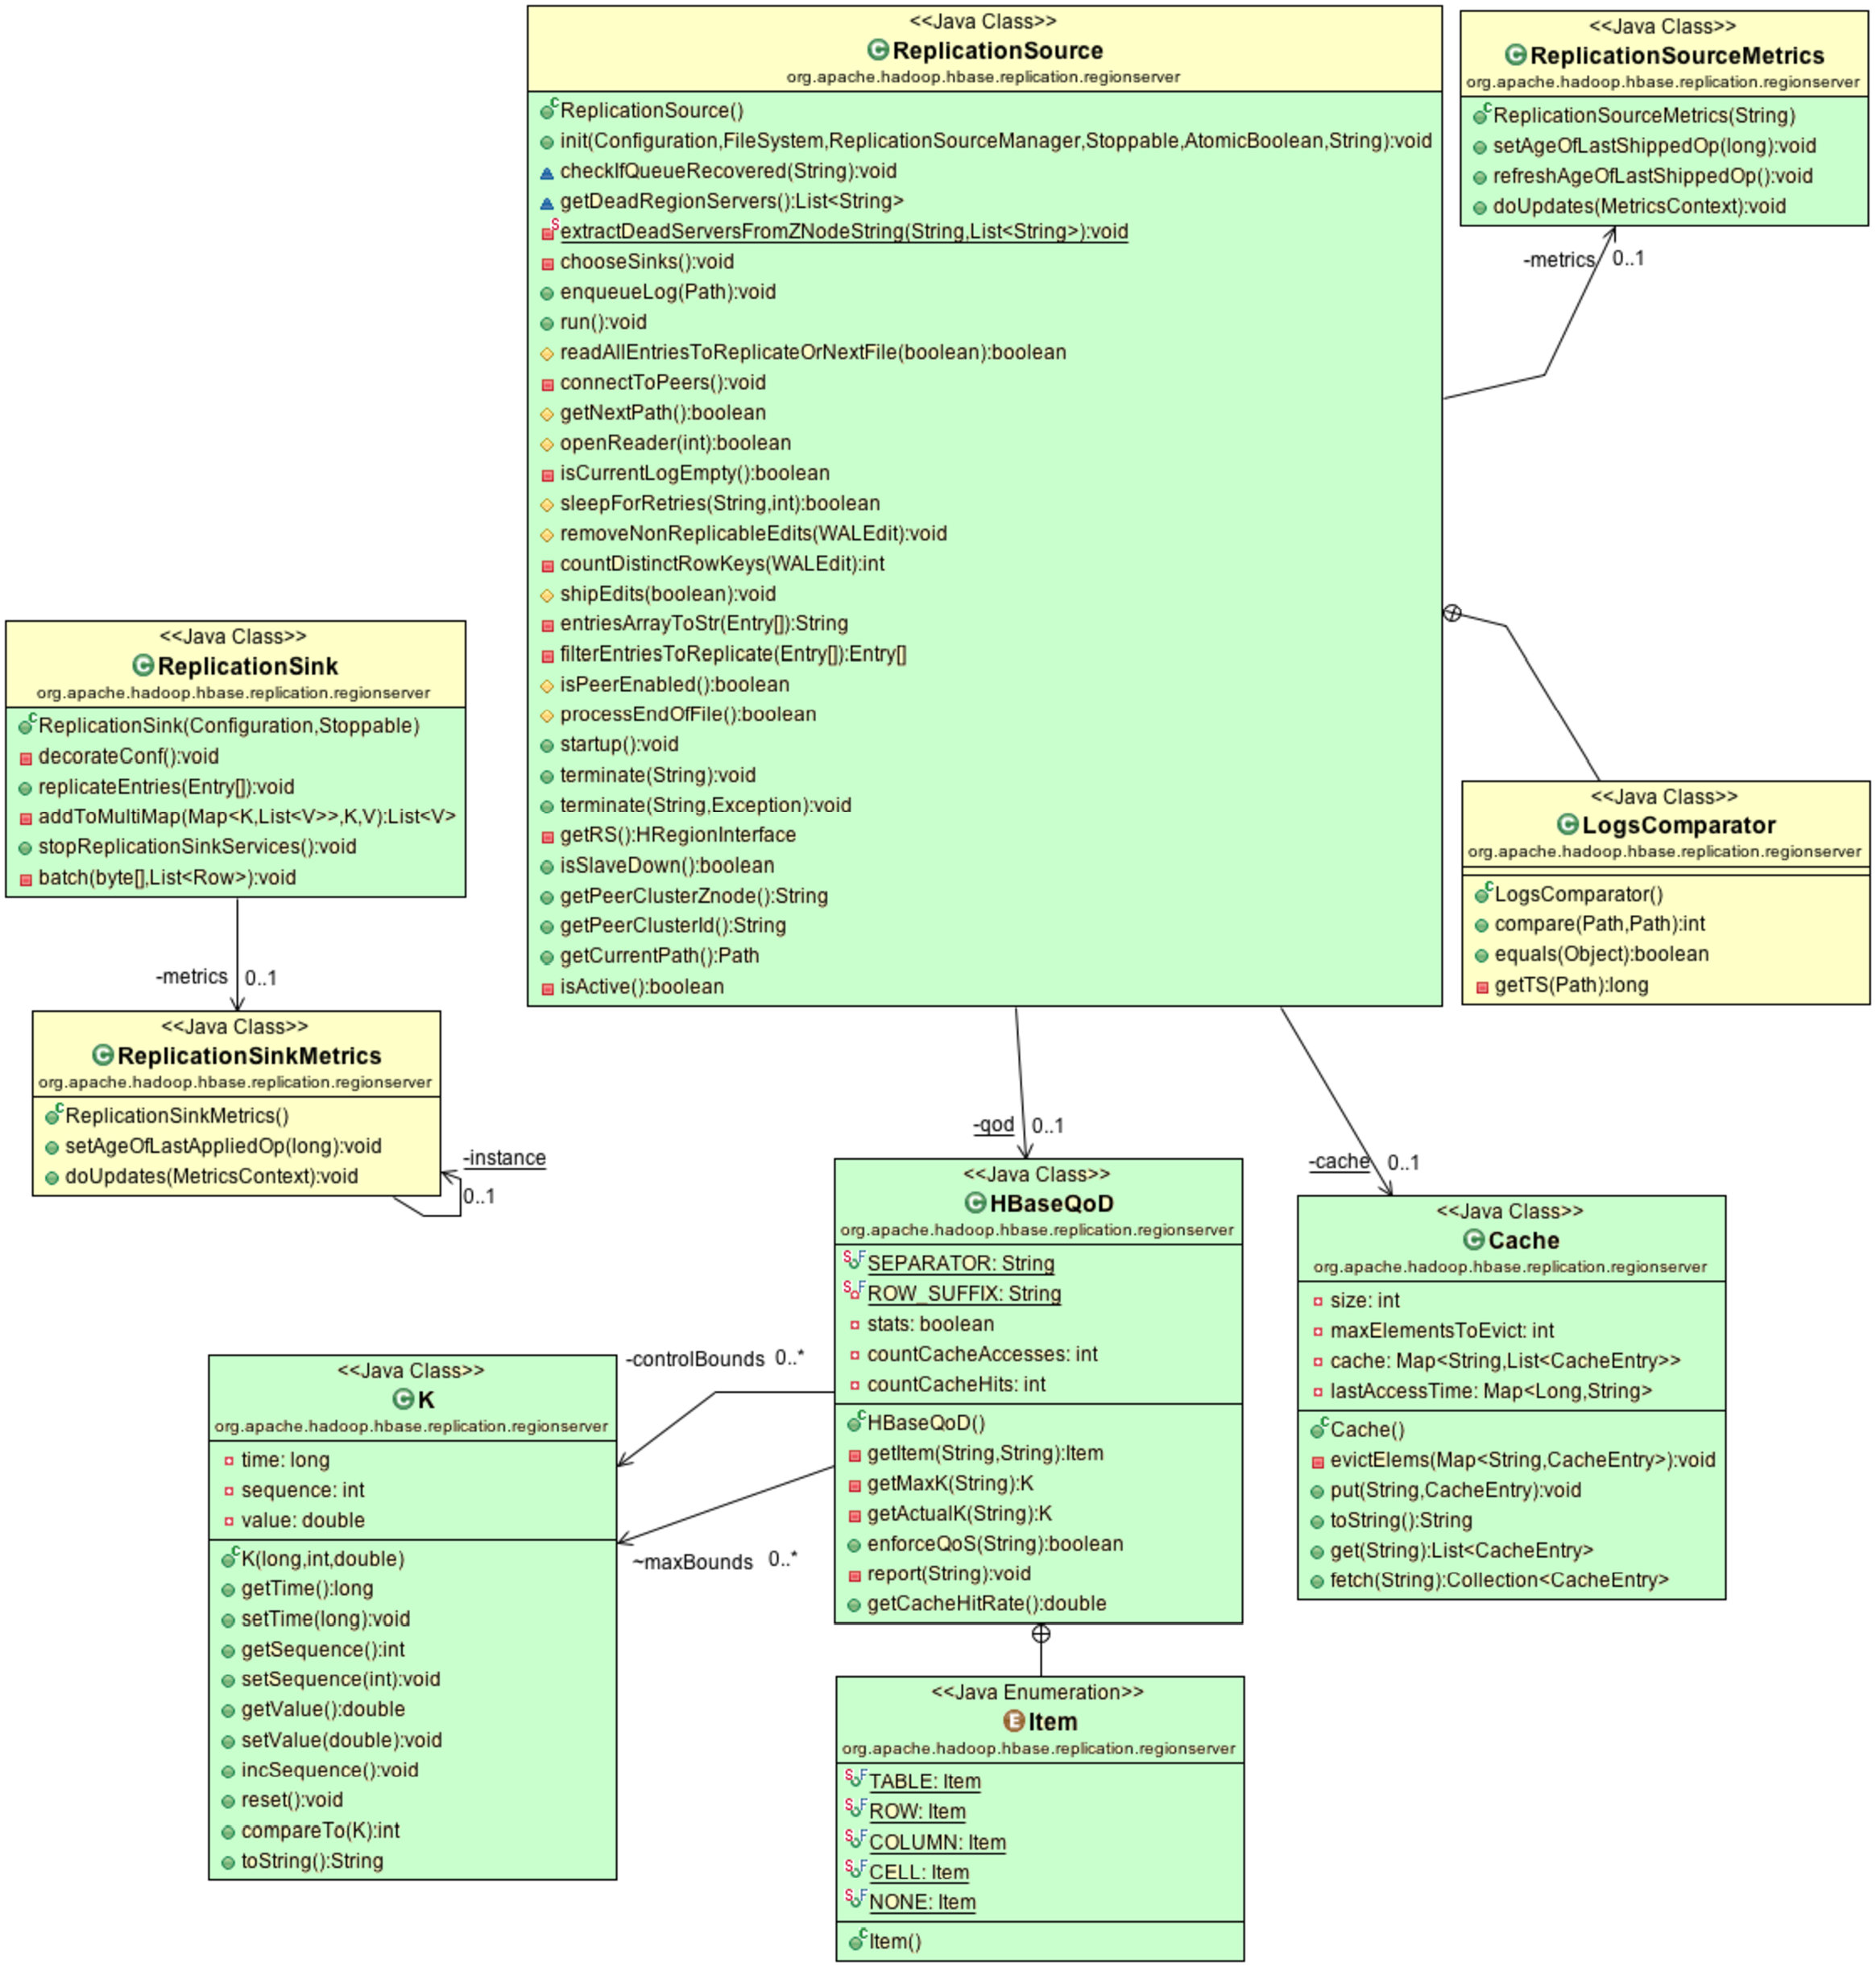
\includegraphics[width=1.0\linewidth]{figs/HBaseQoD-class-diagram.pdf}
\caption{HBase-QoD class diagram}
\label{fig-class-diagram}
\end{figure}

%this may fall into chapter 4, and is a way of making the bridge to the real implementation details in Chap.4.


%(summary)

\section{From eventual consistency to vector-field bounded consistency}\label{architecture:requirements}
This section explains the motivation of the steps taken in regards to the design decisions adopted in order to present an enhanced architecture that also follows best practices in regards to code readability and re-usability for the system of choice. In the following sections of the chapter we justify the 'how' and 'why' of the choices we have made during the development process later once we have a well-rounded architecture of the intended replication module for HBase.

With eventual consistency enforcement in place, updates and insertions are propagated asynchronously between clusters so Zookeeper is used for storing their positions in log files that hold pointers to the next log entry to be shipped in HBase. To ensure cyclic replication (master to master) and prevent from copying same data back to the source, a sink location with remote procedure calls invoked is already into place with HBase. Therefore if we can control the edits to be shipped, we can also decide what is replicated, when or in other words, how soon or often.

\begin{enumerate}
\item Separate concerns in terms of data semantics and replication.
\item Replication is still asynchronous but with a higher degree of consistency guarantees, based on a vector-field consistency model that allows defining the constraints and limits for each type of data then.
\item Partitioning is allowed but eventual consistency allows to reconcile changes autonomously, while grouping of operations enforce maintaining atomically replicated updates so avoiding the first in case of long periods of disconnection to the network (it is already possible to define a retry timeout in HBase in case of partitioning so we do not need to focus on that but rather on the grouping part)
\end{enumerate}

\subsection{Remote Procedure Calls}
HBase implements remote procedure calls for the replication of items between servers or clusters. These mechanisms have been proven a useful paradigm for providing communication across computer networks for several reasons~\cite{Birrell:1984}. An RPC mechanism is mainly responsible for providing control of data transfers between a source and a destination location. In the case of HBase, these are called \emph{ReplicationSource.java} and \emph{ReplicationSink.java} respectively. To understand in depth that topic, it has been discussed in as much depth as possible with Apache Foundation contributors for the HBase community. That is helpful to clarify and understand better how the system operates before introducing the changes proposed with our HBase-QoD.

\section{Challenges addressed and solution proposal}
How long does it take for edits to be propagated to a slave cluster? This is one of the main questions that can strike Cloud Architects when it comes to distributed NoSQL architectures. As noted in the HBase forums, there is a increasing interest in knowing how and when data is propagated to slave clusters. For instance to separate clients facing HBase clusters and the ones used to to run benchmarks and analysis that involves heavy Map Reduce tasks that are very scan intensive.

\paragraph*{Buffering in HBase:}
As noted by Jean-Daniel Cryans, buffering acts as soon as the buffer itself is full or it reaches the end of the file (EOF). The end of a file is determined by when a file is reopened because there is no way to tail a file into HDFS without closing a previous reader, therefore reopening the file and seeking to a certain position it is required. As a consequence, replication is not able to keep filling the buffer for minutes before sending because, as it gets to the EOF quickly either way. The HBase replication stream is almost always in the range of sub-seconds lag. Only if it reaches the end of a file and it does not read anything new, then that will be waiting for new updates to arrive.

In the case of \emph{ReplicationSource}, that tails the WAL and sends the WALEdit to the ReplicationSink via RPC. In other words, the code applies the edits to the slave cluster via a remote call to the method in the RPC sink (calling a method named \emph{ReplicateLogEntries} remotely).

In order to control that, HBase-QoD modifies the internals of buffering WALs at the source that will be sent to a sink location.

\paragraph*{Configurations:}
There is a set of configurations in HBase to control how updates are replicated. That is contained in XML file called hbase-site.xml.

\begin{enumerate}
\item replication.source.size.capacity, default is 64MB but recently so that is possibly too big.
\item replication.source.nb.capacity, default is 25k. The buffer is flushed when either size or capacity is reached but what really important is the size.
\item replication.source.maxretriesmultiplier, default is 10, so it retries up to 10 times with pauses that are currentIteration times.
\item replication.source.sleepforretries. By default it sleeps 1 sec, 2, 3, 4... 9, 10, 10, 10, 10 until it's able to replicate.
\item replication.source.sleepforretries, default is 1 second, see above.
\end{enumerate}

Although useful, currently those mechanisms do not allow to differentiate between application bounds when it comes to flushing updates to slave cluster. Therein the HBase-QoD will show how it can help in that regard.

\section{Development method}\label{method}
In order to introduce a new HBase-QoD module into the previous architecture, we have first studied the system to get familiar with it and identify the best locations for new code added. Therefore we take into account the original programmed inner-workings of the data store logical flow and that ensures correctness and validity of the paradigm implemented later in next chapter. 

\begin{enumerate}
\item First identifying the source and destination of updates.
\item Secondly, defining a QoD vector-model based on the schema design of HBase so we can reach our goals.
\item Finally integrating both parts into the same system, and providing a mechanism to switch on and off the module at run time into HBase.
\end{enumerate}

% Implementation details, such as WALEdit, algorithm, images of QoD inside DC, etc. 
HBase is written in Java and its replication mechanisms are related to a Write Ahead Log (WAL) that also ensures durability of updates and disaster recovery. Replication must be enabled for shipping updates between peer cluster locations in remote or nearby data centers. The process of replication is carried out asynchronously so there is not additional overhead or latency introduced in the the master server during that operation.  Although, since the process is not strongly consistent, in write heavy applications an slave can have stale data in the order of more than just a few seconds according to the eventual consistency approach. Therefore, until the last update first commits to the local disk, it cannot be seen replicated in a remote location. To keep control of staleness, we plug a QoD module called HBase-QoD which provides and takes advantage of a sorted priority queue of update items filtered and scheduled for replication accordingly. Thereafter, when the method completes, updates are shipped in an ordered fashion by enforcing currently defined QoD bound constraints over data marked for delivery to a remote cluster location. For write intensive applications that can be both beneficial in terms of peaks of bandwidth usage and also reduced staleness of data we believe.


Using the QoD involves a temporal caching of updates until the threshold set in the three-dimensional vector is reached, so having a caching mechanism that stores those edits for further evaluation against constraints (namely time, sequence and value) We can then decide if an item or group of items is due to propagation for replication or not.



